

\chapter{روش پیشنهادی}
\tikzstyle{edge_style} = [draw=black,line width=0.3,-latex']
\tikzstyle{line1} = [draw=red,line width=0.3] 
\tikzstyle{line2} = [draw=black,line width=0.3] 
\tikzstyle{operator} = [draw,shape=circle,fill=white,minimum size=1.3em] 
 \tikzstyle{phase} = [draw,shape=circle,minimum size=10pt,inner sep=0pt]
 \tikzstyle{control} = [fill,shape=circle,minimum size=12pt,inner sep=0pt]
 \tikzstyle{hadamard} = [draw,shape=rectangle,fill=black,minimum size=12pt,inner sep=0pt]
\tikzstyle{line} = [draw, -latex']
\tikzstyle{cir1} = [fill=blue!20,shape=circle,minimum size=15pt,inner sep=0pt] 
\tikzstyle{cir2} = [fill=yellow,shape=circle,minimum size=15pt,inner sep=0pt]
\tikzstyle{vertexs}=[draw,minimum width=0pt,minimum height=15pt]
\tikzstyle{cir3} = [fill=green!30,shape=circle,minimum size=15pt,inner sep=0pt]
\algnewcommand\algorithmicforeach{\textbf{for each}}


\algnewcommand\ForEach{\item[ \algorithmicforeach]}
\algdef{S}[FOR]{ForEach}[1]{\algorithmicforeach\ #1\ \algorithmicdo}

\newpage
‎\renewcommand{\baselinestretch}{2}\normalsize‎
\label{proposed approach}
\section{روش پيشنهادي}

 در این فصل، روش پیشنهادی برای ساخت مدار کوانتومی توزیع شده با هدف کاهش تعداد دورنوردی‌های کوانتومی ارائه خواهد شد. در ابتدا مقدمات و کلیات روش شرح داده شده و در ادامه جزئیات هر قسمت بحث خواهد گردید.
\section{مقدمه}
\label{مقدمه}
با توجه به معماری ارائه شده در فصل پیشین، در این رساله برآنیم تا با تمرکز بر لایه دوم، یک مدار کوانتومی از سطح اول دریافت نموده، و بتوانیم آن را بین سیستم‌های کوانتومی به طور مناسب با در نظرگرفتن تعدادی هدف توزیع نماییم. همانطور که در معماری سیستم‌های توزیع شده بیان شد، این مساله از وظایف لایه‌ي دوم می‌باشد. در طراحی این لایه، با چند مساله‌ي اصلی و چالش مواجه هستیم که عبارت‌اند از:
%\begin{figure}[t!]
%\begin{center}
%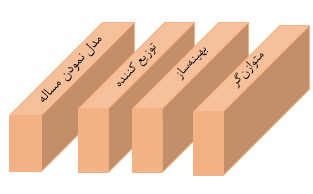
\includegraphics[scale=0.7]{level2.jpg}
%\caption{نیازمندی‌های اصلی در لایه دوم شکل \ref{distribute} }
%\label{level2}
%\end{center}
%\end{figure}
\begin{itemize}
\item
\textbf{ارائه‌ی مدلی مناسب}:
جهت بررسی و طراحی این سیستم، در ابتدا بایستی بتوان آن را به طور دقیق مدل‌سازی نمود و مساله با استفاده از متغیرها و روابط ریاضی توصیف شود. در سطح اول الگوريتم پيشنهادي به مدل‌سازی دقیقي از مساله با استفاده از برنامه ریزی خطی پرداخته شده است.
\item
\textbf{ افرازبند\LTRfootnote{\lr{Partitionner}} یا توزیع کننده}:
پس از مدل‌سازی رياضي، یکی از مهمترین مسائلی که طراحی سیستم‌های کوانتومی توزیع شده با آن مواجه است، استفاده از الگوریتم‌های افرازبندی جهت توزيع كيوبيت‌هاي مدار است. بنابراین یافتن یک الگوریتم جهت افرازبندی مدار امری ضروری است. 
\item
\textbf{بهینه‌ساز\LTRfootnote{\lr{Optimizer}}}:
همانطور که پیش‌تر اشاره شد، از آنجایی‌که تعامل کیوبیت‌ها در محیط با خطا و نویز مواجه است و عملگرهای از راه دور نسبت به عملگرهای محلی بیشتر با این خطاها مواجه هستند، پروتکل دورنوردی عملی هزینه‌بر در سیستم‌های کوانتومی بوده و کاهش تعداد آن امری ضروری است. بنابراین در طراحی این سیستم نیازمند استفاده از الگوریتم بهینه سازی بوده تا بتوان تعداد مورد نظر را بهینه نمود.%یک هدف که کیوبیت‌ها بطور متعادل \lr{\LTRfootnote{Balance}} توزیع شده و تعداد دورنوردی‌های مورد استفاده  جهت ساخت این سیستم حداقل ممکن گردد. بهینه سازی تعداد دورنوردی‌ها در دوسطح انجام میگردد. در سطح اول با ارائه الگوریتمی مدار کوانتومی به $K$ افراز با هدف کاهش تعداد دورنوردی‌ها و توزیع  متعادل کیوبیت‌ها توزیع می‌گردد و در سطح دوم با ارائه‌ی تعدادی قانون این سیستم بهینه‌تر می‌گردد.
\item
\textbf{متوازن‌کننده\LTRfootnote{\lr{Load Balancer}}}:
گاهی اوقات کاهش بیش از اندازه‌ی تعداد پروتکل دورنوردی منجر به عدم توازن در تعداد کیوبیت‌های هر زیر سیستم می‌گردد و از آن‌جایی که هر سیستم‌های کوانتومی دارای محدودیت در تعداد کیوبیت‌ها بوده، همزمان با کاهش تعداد دورنوردی‌های کوانتومی، توزیع متوازن کیوبیت‌ها نیز هدف اصلی قرار می‌گیرد. بنابراین از دیگر مسائلی که در طراحی سیستم‌های کوانتومی توزیع شده با آن مواجه هستیم، مساله‌ی توزیع متوازن بار یا همان توزیع متوازن کیوبیت‌های مدار است. 
\end{itemize}

به دليل پيچيدگي بالاي سيستم‌هاي كوانتومي، طراحي سيستم‌هاي كوانتومي توزيع شده و بهينه‌سازي آن در يك سطح امري دشوار است. راه‌کار پیشنهادی در این رساله این است تا بتوان سیستم مورد نظر را در دو سطح به طور سلسله مراتبی بهینه نمود. این دو سطح عبارت‌اند:
\begin{itemize}
\item

 سطح اول: در این سطح ابتدا مدلی ریاضی از مساله‌ی افرازبندی مدار کوانتومی ارائه خواهد شد. سپس با تبدیل مدار کوانتومی به یک گراف تعداد برش کمینه جهت افرازبندی این مدار به $K$ زیر سیستم بدست خواهد آمد. تعداد برش‌های بدست آمده همان تعداد دروازه‌های سراسری بین سیستم‌ها خواهد بود. در این سطح، زمانبندی اجرای دروازه‌های کوانتومی در نظر گرفته نمی‌شود. خروجي اين سطح برچسب‌گذاري كيوبيت‌ها برحسب شماره افرازي است كه در آن قرار مي‌گيرند.


\item
 سطح دوم: با توجه به افرازبندی بدست آمده از سطح اول، در مرحله‌ی اجرای دروازه‌های سراسری کوانتومی، زمانی که یکی از کیوبیت‌های این دروازه از مبدا خود به مقصد مورد نظر دورنورد می‌گردد، ممکن است کیوبیت دورنورد شده بتواند توسط تعدادی دروازه‌ی سراسری دیگر با رعایت محدودیت‌های پیش نیازی مورد استفاده قرار گرفته و در نتیجه موجب کاهش تعداد دورنوردی‌ها گردد. در این سطح به سوالات زیر پاسخ داده می‌شود: 
\begin{itemize}
\item
زمانی‌که یک کیوبیت از مبدا خود به مقصد دورنورد می‌شود، چه‌زمانی به مقصد خود بازگردد؟ گاهی اوقات با دورنورد شدن یک کیوبیت می‌توان چند دروازه را همزمان اجرا نمود به شرطی که محدودیت‌های پیش نیازی آن‌ها رعایت شده باشند.
\item
در یک دروازه‌ی سراسری دو کیوبیتی، کدام کیوبیت این دروازه دورنورد شود؟  تعداد دروازه‌های سراسری که با دورنورد نمودن کیوبیت کنترلی یا هدف می‌توانند اجرا شوند، در بیشتر موارد متفاوت بوده و در نتیجه پاسخگویی به این سوال امری مهم محسوب می‌گردد.
\end{itemize}
\end{itemize}


\section{متغیرهای مورد استفاده}
مجموعه متغیرهای استفاده شده در این رساله در جدول \ref{notation} آورده شده است.
\begin{table}[h]
\centering
\caption{\small{متغیرهای مورد استفاده در مدل ریاضی }}
\label{notation}
\footnotesize\rm
\begin{tabular}{cc}
\hline
متغیر&توصیف\\
\hline
$N_{g}$&تعداد دروازه‌ها\\
$N_{q}$&تعداد کیوبیت‌ها\\
$run_{i}$&حالت اجرای دروازه‌ی \lr{i}\\
$P_{i}$&شماره افرازی که کیوبیت \lr{i} در آن قرار دارد\\
$N_{t}$&تعداد دورنوردی‌ها\\
$K$&تعداد افرازها\\
$\omega$&نرخ عدم تعادل \\
$N_{non}$&تعداد دروازه‌های سراسری\\
$N_{2qubit}$&تعداد دروازه‌های دوکیوبیتی\\
$\mathcal{G}$&مجموعه دروازه‌های دو کیوبیتی مدار \\
$Q$& مجموعه کیوبیت‌های مدار\\
$QC$& مدار کوانتومی\\
\hline
\end{tabular}
\end{table}

\section{افرازبندی سطح اول}
هدف این سطح این است تا کیوبیت‌های مدار در تعدادی زیر سیستم کوانتومی توزیع شده، به‌طوری‌ که تعداد ارتباط‌ها بین این سیستم‌ها حداقل شود. از آن‌جایی که این مساله \lr{NP-Hard} بوده \cite{andreev2006balanced}، الگوریتمی دقیق با زمان جندجمله‌ای برای آن وجود ندارد. در این سطح در ابتدا به بیان مدلی ریاضی از مساله‌ی افرازبندی مدار کوانتومی پرداخته شده و سپس دو الگوریتم جهت افراز‌بندی کیوبیت‌ها ارائه می‌‌گردد. در الگوریتم اول به توزیع متوازن کیوبیت‌ها در دو زیرسیستم و در الگوریتم دوم به توزیع آن‌ها در چند افراز پرداخته شده است. 
\subsection{مدل‌سازی ریاضی }


تعریف مساله: فرض شود مدار کوانتومی شامل مجموعه‌ای از کیوبیت‌ها $Q=\{q_{i}| i \in\{1,...,N_q\}\}$ و مجموعه‌ای از دروازه‌های دو کیوبیتی مدار $\mathcal{G}=\{g_{j}| j \in\{1,..,N_{2qubit}\}\}$ باشد. جهت مدل سازي اين مساله نياز است كه تعدادی از متغيرهاي دودويي به صورت زير تعريف گردد. 
\abovedisplayskip=3pt
\belowdisplayskip=0pt
\[
p_{i,k}=
\begin{cases}
 1& \text{اگر $q_i$ در افراز $k$ قرار داشته باشد.}\\
0& \text{در غیر اینصورت}
 \end{cases}
\]


\[
f_{j}=
\begin{cases}
 1& \text{اگر دروازه‌ی $g_j$ دروازه‌ای سراسری باشد. }\\
0& \text{در غیر اینصورت}
 \end{cases}
\]


\begin{equation}
\min \sum\limits_{j=1}^{N_{2qubit}} f_{j} 
\label{eq16}
\end{equation}
\begin{equation}
\sum\limits_{i=1}^{N_{q}} p_{i,k} \leq (1+\omega)|Q| /K \quad \forall k=1,...,K
\label{eq17}
\end{equation}

\begin{equation}
\sum\limits_{k=1}^K p_{i,k}=1    \quad \forall i=1,...,N_q
\label{eq18}
\end{equation}

\begin{equation}
f_{j}\geq p_{i_2,k}-p_{i_1,k} \quad \forall k=1,...,K, \quad g_j(i_{1},i_{2}) \in\mathcal{G}
\label{eq19}
\end{equation}

\begin{equation}
f_{j}\geq p_{i_1,k}-p_{i_2,k} \quad \forall k=1,...,K, \quad g_j(i_{1},i_{2}) \in\mathcal{G}
\label{eq20}
\end{equation}

 $f_{j} \in\{0,1\}, p_{i_1,k}\in\{0,1\} \quad \forall i=1,...N_{q}, j=1,...,N_{2qubit}, k=1,...,K$

 این رابطه‌ها به ترتیب در زیر تعریف شده‌اند:
\begin{itemize}
\item
رابطه \eqref{eq16} تابع هدف را نشان می‌دهد که این تابع به‌دنبال کمینه نمودن تعداد ارتباط‌‌ها در مدار یا همان تعداد دروازه‌های سراسری است.
\item
رابطه‌ی \eqref{eq17} شرط توزیع شدن متوازن کیوبیت‌ها را نشان می‌دهد. در این رابطه مجموع تعداد کیوبیت‌هایی که در یک افراز قرار می‌گیرد، بایستی از مقدار $(\frac{1+\omega}{K}|Q|)$ کمتر یا مساوی باشد.
\item

رابطه \eqref{eq18} بیانگر این است که هر کیوبیت تنها به یک افراز تخصیص یابد. 
\item
در رابطه‌های \eqref{eq19} و \eqref{eq20} شرط این‌که دوکیوبیت در دو افراز جدا قرار گرفته باشند و تشکیل یک دروازه‌ی سراسری بدهند، بررسی می‌گردد.
\end{itemize}




 
\subsection{الگوریتم توزیع کیوبیت‌ها در دو افراز}
الگوریتم ژنتیک یکی از الگوریتم‌های اکتشافی حل مسئله است که از مدل‌سازی زیستی جمعیت جانداران به‌وجود آمده است. در این الگوریتم، خصوصیات نسل جانداران به مقدار توابع هدف و بهبود در خصوصیات نسلی در پی گذشت زمان تشبیه و ظهور نسل‌های جدید از آمیزش نسل‌های قبلی به بهبود در مقدار توابع هدف مانند شده است. به‌عبارت دیگر این الگوریتم از اصول انتخاب طبیعی داروین برای یافتن فرمول یا جواب بهینه به منظور پیش‌بینی یا تطبیق الگو استفاده می‌کند. الگوریتم  \LTRfootnote{\lr{Non-Dominated Sorting Genetic Algorithm}}\lr{NSGA-III} یکی از روش‌های حل چند هدفه‌ی الگوریتم ژنتیک است. در این بخش با استفاده ازین الگوریتم به توزیع متوازن کیوبیت‌ها در دو افراز پرداخته شده است. این الگوریتم یکی محبوب‌ترین روش‌های حل مسائل بهینه‌سازِی چندهدفه است. این الگوریتم از مراحل زیر تشکیل شده است:
\begin{itemize}
\item
ایجاد جمعیت اولیه
\item
محاسبه‌ی معیارهای برازندگی\LTRfootnote{\lr{Fitness function}}
\item
مرتب کردن جمعیت براساس شرط‌های غلبه کردن\LTRfootnote{\lr{Dominate}}
\item
محاسبه فاصله‌ی ازدحامی\LTRfootnote{\lr{Crowding Distance}}
\item
انتخاب\LTRfootnote{\lr{Selection}}: به محض اینکه جمعیت اولیه بر اساس شرط‌های غلبه کردن مرتب شد، مقدار فاصله‌ی ازدحامی در آن محاسبه خواهد شد و انتخاب از میان جمعیت اولیه آغاز می‌شود. این انتخاب بر اساس دو عملگر  زیر صورت می‌گیرد:
\begin{itemize}
\item
رتبه‌ی جمعیت\LTRfootnote{\lr{Population ranking}}: جمعیت‌ها در رتبه‌ی پایین انتخاب می‌شوند.
\item
محاسبه‌ی فاصله:
با فرض این‌که \lr{p} و \lr{q} دو عضو از یک رتبه باشند، عضوی انتخاب می‌شودکه فاصله‌ی ازدحامی بیشتری دارد. اولویت انتخاب، ابتدا با رتبه و سپس بر اساس فاصله‌ی ازدحامی است.
\end{itemize}
\item
انجام تقاطع \LTRfootnote{\lr{Crossover}} و جهش \LTRfootnote{\lr{Mutation}} برای تولید فرزندان جدید.
\item
تلفیق جمعیت اولیه و جمعیت به‌دست آمده از تقاطع و جهش.
\item
جایگزین نمودن جمعیت والدین با بهترین اعضای جمعیت تلفیق شده در مراحل قبل. 
\end{itemize}
\subsection{هدف‌ها}
\begin{itemize}
\item
هدف‌هایی که در این الگوریتم به دنبال بهینه‌سازی آن هستیم، عبارت‌اند از:
کمینه نمودن تعداد دروازه‌های سراسری در توزیع بدست آمده\lr{(GlobalNum)}: از آنجایی که هدف از افرازبندی کیوبیت‌ها، کاهش تعداد دورنوردی‌های کوانتومی است، كمينه نمودن تعداد دروازه‌های سراسری منجر به کاهش تعداد دورنوردی‌های کوانتومی می‌گردد. 
\item
کمینه نمودن اختلاف تعداد کیوبیت‌های بدست آمده در دو افراز \lr{(QNum)}: همانطور که قبلا بیان شد، یکی از چالش‌های اساسی در این سیستم این است که توزیع کیوبیت‌ها در افرازهای متفاوت، متعادل باشد. بنابراین هر چه اختلاف کیوبیت‌های قرار گرفته در دو افراز به صفر نزدیک باشد، نشان دهنده‌ی توزیع متوازن آن‌ها خواهد بود. بنابراین این پارامتر به عنوان هدف دوم در الگوریتم ارائه شده در نظر گرفته خواهد شد. 
\end{itemize}
\subsection{ساختار کروموزوم}
طول کروموزوم بکار رفته در این الگوریتم برابر $N_q+1 $ می‌باشد. در این الگوریتم پارامتری به نام خط برش یا \lr{Cutline} تعریف شده است که بیانگر محلی است که کیوبیت‌ها از یکدیگر جدا شده و در دو افراز قرار می‌گیرند. همچنین مقادیر ژن‌های کروموزوم به صورت زیر مقداردهی شده است:
\begin{itemize}
\item
ژن اول بیانگر مکان خط برش می‌باشد. 
\item
ژن \lr{i+1} متناظر با مکان کیوبیت \lr{i}ام در توزیع بوجود آمده می‌باشد.
\end{itemize}
 
 با توجه به موارد بیان شده به تعداد \lr{Cutline} کیوبیت در افراز اول و به تعداد \lr{$N_q$-Cutline} کیوبیت در افراز دوم قرار گرفته است. برای توضیح بیشتر در ادامه به بیان مثالی پرداخته شده است. شکل \ref{fig:a} یک مدار کوانتومی با شش کیوبیت را نشان داده و نمونه‌ای از یک کروموزوم متناظر با اين مدار، در شکل \ref{chromeelahi} آورده شده است. 
 \begin{figure}
 \centering
\includegraphics[scale=0.7]{chromeelahi.jpg}
\caption{نمونه‌ای از کروموزوم مورد استفاده در الگوریتم }
\label{chromeelahi}
 \end{figure}
 در این کروموزوم مکان خط برش در محل 2 قرار گرفته و کیوبیت‌های 1 تا 6 به‌ترتیب در مکان‌های 3، 1، 2، 5، 6 و 4 قرار گرفته است. مدار بدست آمده در شکل \ref{fig:b} آورده شده است.
 \begin{figure}[h]
\centering     
\subfigure[مدار کوانتومی اولیه]{\label{fig:a}\includegraphics[width=130mm]{elahisample1}}
\subfigure[چگونگی توزیع کیوبیت‌ها در دوافراز با توجه به کروموزوم ارائه شده در شکل \ref{chromeelahi}]{\label{fig:b}\includegraphics[width=130mm]{elahisample2}}
\caption{چگونگی توزیع کروموزوم‌ها با استفاده از الگوریتم \lr{NSGA-III} در دو افراز}
\label{elahisample}
\end{figure}

بعد از اعمال الگوریتم \lr{NSGA-II} روی مدار مورد نظر، جواب بهینه‌ي بدست آمده همانند مدار شکل \ref{optimalelahi} است.  در جواب بهینه‌‌ی بدست آمده کیوبیت‌های $q_4 $، $q_1 $ و $q_6 $ در افراز اول و کیوبیت‌های $q_3 $، $q_2 $ و $q_5 $ در افراز دوم قرار گرفته‌اند. همچنین مقادير پارامترهای \lr{Qnum} و \lr{GlobalNum} به‌ترتيب برابر با 0 و 4 بدست آمده است.
 \begin{figure}[h]
\centering     
\subfigure[مدار کوانتومی بدست آمده پس از اعمال الگوریتم \lr{NSGA-III}]{\label{figa}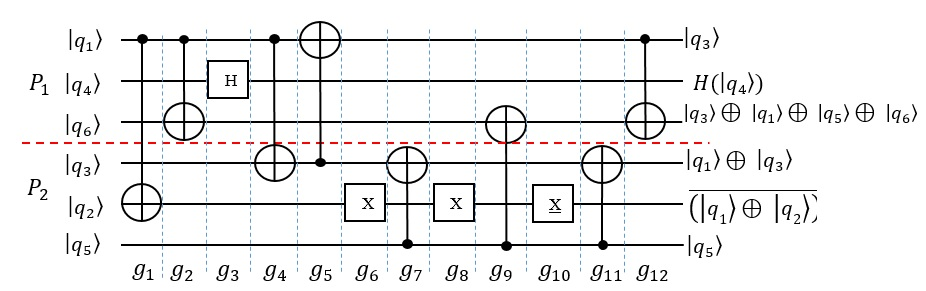
\includegraphics[width=130mm]{optimalelahi}}
\subfigure[کروموزوم بدست آمده]{\label{figb}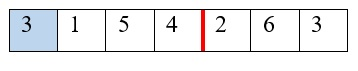
\includegraphics[width=60mm]{optimalelahich}}
\caption{جواب بهینه بدست آمده پس از اعمال الگوریتم \lr{NSGA-III} روی مدار شکل \ref{fig:a}}
\label{optimalelahi}
\end{figure}

\subsection{الگوریتم پیشنهادی جهت افرازبندی چندگانه }
در این قسمت به مساله‌ی افرازبندی کیوبیت‌ها در چند افراز پرداخته شده و براي حل آن از برنامه‌سازی پویا\LTRfootnote{\lr{Dynamic Programming}} استفاده گرديده است. الگوریتم1 ساختار اصلی راه حل پیشنهادی در این مرحله را نشان می‌دهد. این الگوریتم مدار کوانتومی داده شده در ورودی مساله را با هدف کاهش تعداد دورنوردی‌های مورد نیاز و در نظر گرفتن توازن افرازها، در $K$ افراز توزیع نموده و از دو مرحله تشکیل شده است: در مرحله‌ی اول سعی شده است بتوان مدار کوانتومی را به شکل یک گراف دو بخشی نمایش داد (خط 4 تابع \lr{QCtoBigraph}) و سپس در مرحله‌ی دوم با استفاده از برنامه‌سازی پویا، الگوریتمی جهت افرازبندی گراف دو بخشی ارائه گردد (خط 5 تابع \lr{DP}). خروجي اين الگوريتم تعداد دروازه‌هاي سراسري و آرايه‌ي $P$ است كه بيانگر شماره افرازهايي است كه هر كيوبيت به آن تعلق گرفته است.

\begin{algorithm}
{
\fontsize{9}{1}
\caption{$\text{: الگوریتم اصلی جهت افرازبندی مدار کوانتومی در چند افراز}$}
\begin{algorithmic}[1]
\begin{latin}
\Function {Main} {QC, K}

\State\textcolor[rgb]{0.00,0.50,1.00}{ $\triangleright$ \lr{Input: Quantum Circuit (QC), The number of partitions ($K$)}}
\State\textcolor[rgb]{0.00,0.50,1.00}{ $\triangleright$ Output: The minimum number of non-local gates, P }
\State \textcolor[rgb]{0.00,0.50,1.00}{ $\triangleright$ Step I:} G=QCtoBigraph(QC);
\State \textcolor[rgb]{0.00,0.50,1.00}{ $\triangleright$ Step II:}  $N_{non}$=DP(G,K);

\EndFunction
\end{latin}
\end{algorithmic}
}

\end{algorithm}

\begin{itemize}
\item
\textbf{مرحله‌ي اول:}
در این مرحله، مدار کوانتومی به صورت یک گراف دو بخشی نشان داده می‌شود. به طوری که مجموعه دروازه‌های مدار، در یک سمت گراف دو بخشی (بخش \lr{Y}) و در سمت دیگر آن (بخش \lr{X}) مجموعه کیوبیت‌های موجود در مدار کوانتومی قرار می‌گیرند. یال‌های اين گراف شامل دروازه‌های دو کیوبیتي مدار هستند و به صورت زیر ایجاد می‌گردند:

به ازای هر دروازه‌ی دو کیوبیتی $g_{j}(q_{c},q_{t})$، دو یال $(g_{j},q_{t})$ و $(g_{j},q_{c})$ به گراف اضافه می‌گردند. از آنجایی‌که دروازه‌های تک کیوبیتی تاثیری در افرازبندی گراف ندارند، در این مرحله از روش آن‌ها از مدار حذف شده و در نظر گرفته نمی‌شوند. 

الگوریتم 2 چگونگی تشکیل این گراف دو بخشی را نشان می‌دهد.

 \begin{algorithm}
{
\fontsize{9}{1}
\caption{$\text{: چگونگی تبدیل مدار کوانتومی به گراف دو بخشی}$}
\begin{algorithmic}[2]
\begin{latin}
\Function {G=QCtoBigraph} {QC}
\State\textcolor[rgb]{0.00,0.50,1.00}{ $\triangleright$   Step I: Convert QC to Bigraph}
\State Initialize G(V,E) ,   $G.X=Q$  ,  $G.Y=\mathcal{G}$ and   $ E=\{\}$ ; \textcolor[rgb]{0.00,0.50,1.00}{ $\triangleright$ $ V=X \cup Y$}
\State\textcolor[rgb]{0.00,0.50,1.00}{ $\triangleright$  Qubits are in one part of bigraph G (part X) and gates are in the other parts ( part Y)  }
   \For {each $ g_{j} \in \mathcal{G}$}
         \State $q_c\leftarrow$ contorol qubit of $g_{j}$;
        \State $q_t \leftarrow$ target qubit of $g_{j}$;
         \State  Add to $E$ edges $(q_c,g_{j})$ and $(q_t,g_{j})$;
 \EndFor
\EndFunction
\end{latin}
\end{algorithmic}
}
\end{algorithm}

در این الگوریتم در ابتدا یک گراف دوبخشی به نام \lr{G} با دو مجموعه‌ی تهی \lr{X} و \lr{Y} و بدون یال در نظر گرفته مي‌شود. روشن است که اجتماع دو مجموعه‌ی \lr{X} و \lr{Y} مجموعه رئوس گراف یا همان مجموعه‌ی \lr{V} را تشکیل می‌دهند. سپس به ازای هر $g_j \in \mathcal{G}$ مجموعه یال‌های ذکر شده در بالا به یال‌های گراف اضافه خواهد شد. برای مثال گراف دو بخشی  مدار ارائه شده در شکل \ref{10}، در شکل \ref{11} نشان داده شده است.
\begin{figure}
\begin{center}

    \begin{tikzpicture}
    \node at (0,0) (q1) {\ket{q_{1}}};    \node at (0,-1) (q2) {\ket{q_{2}}};    \node at (0,-2) (q3) {\ket{q_{3}}};    \node at (0,-3) (q4) {\ket{q_{4}}};
    \node[control] (c20) at (2,0) {} ;edge [-] (q1);    \node[operator] (r21) at (2,-1) {} ;edge [-] (q2);    \draw[-] (2,-1.3) -- (c20);

 % Column 3
    \node[control] (c31) at (3,-1) {};    \node[operator] (r33) at (3,-2) {};    \draw[-] (c31) -- (3,-2.3);

 % Column 4
    \node[control] (r40) at (4,0) {} ;    \node[operator] (c42) at (4,-2) {};    \draw[-] (4,-2.3) -- (r40);

   % Column 5
    \node[operator] (r52) at (5,-2) {} ;    \node[control] (c53) at (5,-3) {};   \draw[-] (5,-1.7) -- (c53);
    %
   
% Column 6
    \node[control] (r62) at (6,-2) {} ;    \node[operator] (c63) at (6,-3) {};    \draw[-] (6,-3.3) -- (r62);

%Column 7
 \node[control] (r71) at (7,-1) {} ;    \node[operator] (c72) at (7,-2) {};    \draw[-] (7,-2.3) -- (r71);

%Column 8
 \node[control] (r82) at (8,-2) {} ;    \node[operator] (c83) at (8,-3) {};    \draw[-] (8,-3.3) -- (r82);

 \node (end1) at (9,0) {} edge [-] (q1);\node (end2) at (9,-1) {} edge [-] (q2); \node (end3) at (9,-2) {} edge [-] (q3); \node (end4) at (9,-3) {} edge [-] (q4);

\draw [line2,dashed](2.5,0.5)-- (2.5,-4);
\draw  [line2,dashed](3.5,0.5)-- (3.5,-4);
\draw  [line2,dashed](4.5,0.5)-- (4.5,-4);
\draw  [line2,dashed](5.5,0.5)-- (5.5,-4);
\draw  [line2,dashed](6.5,0.5)-- (6.5,-4);
\draw  [line2,dashed](7.5,0.5)-- (7.5,-4);
  \node at (2,-4)  {$g_{1}$};  \node at (3,-4)  {$g_{2}$};  \node at (4,-4)  {$g_{3}$};  \node at (5,-4)  {$g_{4}$}; 
 \node at (6,-4)  {$g_{5}$};  \node at (7,-4)  {$g_{6}$};   \node at (8,-4)  {$g_{7}$}; 
 \end{tikzpicture}
\end{center}
\caption{مثالی از مدار کوانتومی }
\label{10}
\end{figure}

\begin{figure}[t!]
\begin{center}
\begin{tikzpicture} 
\vertexs [cir2](a1) at (3,0) []{$q_{1}$};\vertexs [cir2](a2) at (4.5,0) []{$q_{2}$};\vertexs [cir2](a3) at (6,0) []{$q_{3}$};\vertexs [cir2](a4) at (7.5,0) []{$q_{4}$};
\vertex[cir3] (b1) at (0,2) []{$g_{1}$};\vertex [cir3](b2) at (1.5,2) []{$g_{2}$};\vertex [cir3](b3) at (3,2) []{$g_{3}$};\vertex [cir3](b4) at (4.5,2) []{$g_{4}$};
\vertex [cir3](b5) at (6,2) []{$g_{5}$};\vertex [cir3](b6) at (7.5,2) []{$g_{6}$};\vertex [cir3](b7) at (9,2) []{$g_{7}$};
\path
(a1)edge(b1)  (a2)edge(b1)  (a2)edge(b2)  (a3)edge(b2) (a1)edge(b3)  (a3)edge(b3)  (a3)edge(b4) (a4)edge(b4) (a3)edge(b5) (a4)edge(b5) (a2)edge(b6) (a3)edge(b6) (a3)edge(b7) (a4)edge(b7);
\end{tikzpicture}
\caption{گراف دو بخشی مدار کوانتومی ارائه شده در شکل \ref{10}}
\label{11}
\end{center}
\end{figure}

\item
\textbf{مرحله‌ي دوم:}
در این مرحله با ارائه یک الگوریتم برنامه‌سازی پویا سعی شده است تا کیوبیت‌هایی که در یک سمت گراف دو بخشی قرار گرفته‌اند، با هدف کاهش تعداد ارتباط‌ها در تعداد $K$ زیر سیستم متعادل توزیع شوند. 

ساختار درخت بازگشتی برای حل مساله در شکل \ref{12} نشان داده شده است. عمق این درخت برابر با تعداد افرازهای مساله می‌باشد. در هر سطح از درخت کیوبیت‌های یک افراز مشخص شده و مقداردهی می‌گردد. سپس برای مجموعه کیوبیت‌های باقی‌مانده این عمل در سطوح پایین‌تر درخت تکرار می‌گردد. 
\begin{figure}
    \begin{tikzpicture}
%\draw [line,dashed][rotate around={20:(-6,-3)},red] (-6,-3) ellipse (90pt and 20pt);
   \node at (-4,0) (q1) {$T(S_{n},i)$}; \node at (-8,-2) (q2) {$T(S_n-S^{'}_{\lceil{\frac{n}{i}}\rceil},i-1)$}; \node at (-4,-2) (q3) {$T(S_n-S^{'}_{\lceil{\frac{n}{i}}\rceil},i-1)$}; \node at (0,-2) (q4) {...};
 \node at (3,-2) (q5) {$(S_n-S^{'}_{\lceil{\frac{n}{i}}\rceil},i-1)$}; 
 \node at (-11,-4) (q6) {$T(S_n-S^{'}_{2\times\lceil{\frac{n}{i}}\rceil},i-2)$}; \node at (-8,-4) (q7) {...};
\node at (-4,-4) (q9) {$T(S_n-S^{'}_{2\times\lceil{\frac{n}{i}}\rceil},i-2)$};\node at (-2,-4) (q10) {...};
\path[edge_style](q1)edge(q2);\path[edge_style](q1)edge(q3);\path[edge_style](q1)edge(q4);\path[edge_style](q1)edge(q5);\path[edge_style](q2)edge(q6);
\path[edge_style](q2)edge(q7);\path[edge_style](q3)edge(q9);\path[edge_style](q3)edge(q10);
\end{tikzpicture}  
\caption{ساختار درخت بازگشتی مساله با استفاده از برنامه‌سازی پویا}
\label{12}
\end{figure}
مساله‌ي اصلی در ریشه‌ی این درخت قرار دارد که به‌صورت $T(S_n,i)$ تعریف می‌گردد. این مقدار بیان‌گر حداقل تعداد ارتباط‌های مورد نیاز جهت افراز‌بندی مجموعه‌ی $S$ با اندازه‌ی $n$ در $i$ افراز مختلف است به طوری‌که مجموعه‌ی $S$ بیان‌گر کل کیوبیت‌های مدار بوده که در بخش $X$ از گراف دو بخشی قرار گرفته است. در این درخت بازگشتی هرجا از مجموعه‌ی $S$ و $S^{'}$ استفاده شده، اندازه‌ی آن به عنوان اندیس در زیر آن نوشته شده است. از آنجایی که تعداد کیوبیت‌ها در هر افراز بایستی متعادل باشد، در هر سطح از درخت زیر مجموعه‌هایی از $S$ انتخاب می‌گردد که در از حد بالا و پایین بیان شده در رابطه‌ی \eqref{eq28} صدق نمایند. این حد بالا و پایین بر اساس رابطه‌ی \eqref{eq15} در فصل اول و نرخ توزیع توازن بار بیان شده است.

رابطه‌ی بازگشتی ارائه شده برای حل مساله در \eqref{eq28} آورده شده است:
\begin{center}
\begin{equation}
\begin{split}
T(S,i)=min_{S^{'} \subset S }( Connect(S^{'}, S-S^{'})+T(S-S^{'},i-1))\\
\text{به‌طوری‌که}\\
   1< i\leq K\\
|S|-\lceil(1+\omega)\frac{|Q|}{K})\rceil(i-1) \leq|S^{'}| \leq \lceil(1+\omega)\frac{|Q|}{K}\rceil\\
\end{split}
\label{eq28}
\end{equation}
\end{center}



فرض شود که کیوبیت‌های مدار در مجموعه‌ی \lr{S}  قرار گرفته و این کیوبیت‌ها می‌خواهند در $i$ زیر سیستم توزیع شوند. بنابراین رابطه‌ی اصلی به صورت \lr{T(S,i)} فراخوانی می‌گردد. این رابطه از دو قسمت تشکیل شده است. قسمت اول آن انتخاب زیرمجموعه‌ای مناسب به نام $S^{'}$ بوده و اندازه‌ی این زیر مجموعه بایستی دارای دو ویژگی زیر باشد:
\begin{itemize}
\item
اندازه‌ی زیر مجموعه‌ی $S^{'}$ بایستی دارای حد بالای \lr{$(1+\omega)\frac{|Q|}{K}$} باشد.
\item
 توجه به تعیین حد بالا برای اندازه‌ی مجموعه‌ی $S^{'}$، بایستی حد پایینی برای آن نیز در نظر گرفت. از آنجایی که بایستی تعداد کیوبیت‌های سایر زیرسیستم‌ها از حد بالای بیان شده در مورد اول بیشتر نشود، در هر مرحله، حد پایین زیر مجموعه‌ی $S^{'}$ بایستی در رابطه‌ی \eqref{eq29} صدق نماید. 
\begin{equation}
|S|-\lceil(1+\omega)\frac{|Q|}{K}\rceil(i-1) \leq|S^{'}|
\label{eq29}
\end{equation}

\end{itemize}

همانطور که پیشتر بیان گردید، انتخاب اندازه‌ی مناسب برای مجموعه‌‌ی  $S^{'}$  به معنای تعداد کیوبیت‌هایی است که در یک زیرسیستم قرار می‌گیرند. ار آنجایی‌که هر زیرسیستم دارای ظرفیت محدودی از لحاظ تعداد کیوبیت‌ها است، انتخاب مناسب اندازه‌ی آن در توزیع متوازن کیوبیت‌ها و تعداد دورنوردی‌های کوانتومی تأثیر می‌گذارد.
قسمت دوم این تابع بازگشتی، شمارش تعداد دروازه‌های سراسری بین دو زیر مجموعه‌‌ی $S^{'}$ و $S-S^{'} $ می‌باشد. به عبارتی هر دورازه‌ای که بین مجموعه‌ کیوبیت‌های مجموعه‌ی $S^{'}$ و $S-S^{'} $ در گراف دو بخشی وجود دارد، یک دروازه‌ای سراسری است و دروازه‌ی سراسری نیاز به برقراری ارتباط بین دو زیرمجموعه‌ی $S^{'}$ و $S-S^{'} $ دارد. محاسبه‌ی تعداد دروازه‌های سراسری بیان شده، با استفاده از تابعی به‌نام $Connect$ انجام می‌شود. این تابع در رابطه‌ی \eqref{eq261} نشان داده شده است.


\begin {equation}
 Connect (S_{1},S_{2})=| Global\_gate(q_{t},q_{c})|
\label{eq261}
\end{equation}
\begin{center}
\begin{latin}
 $S.t$      ($q_{t} \in S_{1}$  and  $q_{c}\in S_{2}$)    $or$       ($q_{c} \in S_{1}$ and  $q_{t}\in S_{2}$)
 \end{latin}
\end{center}
\end{itemize}
بخش سوم تابع، شامل فراخوانی بازگشتی تابع بوده که به‌صورت $T(S-S^{'},i-1)$ فراخوانی می‌گردد. به عبارتی باقیمانده‌ی کیوبیت‌های مدار بایستی در $i-1 $ زیرسیستم توزیع شوند. 
در این رابطه‌ی بازگشتی، دو شرط توقف زیر وجود دارد:
\begin{itemize}

\item
 چنان‌چه مقدار $i=1 $ بوده و اندازه‌ی مجموعه \lr{S}  حداکثر \lr{$(1+\omega)\frac{|Q|}{K}$} باشد، مقدار$T(S,i)$ برابر صفر قرار می‌گیرد.
\item
چنان‌چه در هر سطح از درخت در محاسبه \lr{$T(S,i)$} محدودیت $\frac{|S|}{i} \leq (1+\omega)\frac{|Q|}{K}$ نقض گردید، درخت هرس شده و مقدار آن برابر بی‌نهایت قرار می‌گیرد. زیرا حداقل تعداد کیوبیت‌های یکی از افرازها از مقدار حد بالای ممکن و ظرفیت خود تجاوز نموده و شرط توازن بار رعایت نمی‌گردد.
\end{itemize}

الگوریتم سه ساختار کلی الگوریتم برنامه‌سازی پویا را نشان می‌دهد. خروجی این سطح برچسب‌گذاری کیوبیت‌ها در افرازی است که به آن تعلق گرفته‌اند و این اطلاعات در آرایه‌ی $P$ قرار گرفته تا به ورودی سطح بعدی جهت بهینه‌سازی تعداد دورنوردی‌های مورد نیاز داده شود.


\begin{algorithm}[t]
{
\fontsize{9}{1}
\caption{$\text{: الگوریتم برنامه‌سازی پویا جهت افرازبندی مدار کوانتومی}$}
%\label{fig4}
\begin{algorithmic}[3]
\begin{latin}
\Function{$N_t$=DP} {G,k}

\State\textcolor[rgb]{0.00,0.50,1.00}{ $\triangleright$ Step II: DP approach to find minimum number of  teleportation}
\State Initialize set $S$ with member of $X$ of graph $G$
\If {$k==1$ }
\State $Return$  0;
\EndIf
\State $index$= Comupte decimal number of S;
\State $ C[index,k]=\infty$;
\For {each $S^{'} \subset S$  }
    \State $q=connect(S^{'},S-S^{'})+DP(S-S^{'},k-1)$;
   \If  {$q\leq C[index,k]$}
       \State $C[index,k]=q$;
   \EndIf
\EndFor
\State $Return$  $C[index,k]$;
\EndFunction
\Function {count=Connect}{$S_{1},S_{2}$}
\State \textcolor[rgb]{0.00,0.50,1.00}{ Output:The number of global gates between $S_{1}$  and $S_{2}$}
\State $count=0$;
\For{ each $q_{i}  \in S_{1}$}
\For{  each $q_{j} \in S_{2}$}
\For { each $g_{k} \in \mathcal{G}$}
 \If{$(g_{k},q_{i}) \in E$  and $(g_{k},q_{j}) \in E$}
     \State $count++$;
\EndIf
\EndFor
\EndFor
\EndFor
\State $Return$ $count$;
\EndFunction

\end{latin}
\end{algorithmic}
}
\end{algorithm}


 %مقدار بدست آمده از $T(S,k)$ در جدولی به‌نام $C$ و در محل $C[index,k]$ ذخیره می‌شود. 
\section{بهینه‌سازی سطح دوم}

در سطح دوم، نیاز به بررسی دقیق‌تر مدار کوانتومی است. زیرا در این سطح بایستی اولویت‌ها و محدوديت‌هاي پیش نیازی جهت اجرای هر دروازه بررسی گردد. بنابراین نیاز است تا اطلاعاتی نظیر کنترل یا هدف بودن کیوبیت‌ها در ورودی‌های هر دروازه در دسترس باشد. برخلاف سطح قبل که نیازی به این اطلاعات برای هر دروازه نبوده است. در این سطح برچسب‌گذاری کیوبیت‌ها که هر کدام در چه افرازی قرار گرفته است و از سطح اول بدست آمده است، به عنوان ورودی در نظر گرفته می‌شود. برای این منظور آرایه‌ای به نام  \lr{$P$} با اندازه \lr{$N_q$} تعریف نموده که مقدار عنصر \lr{$P_{i}$} بیانگر شماره افرازی است که کیوبیت \lr{$i$} در آن قرار گرفته است.

جهت نمایش مدار کوانتومی ماتریسی به‌نام $C$ با ابعاد $N_q*N_g$ در نظر گرفته شده است. عناصر این ماتریس به صورت زیر مقداردهی می‌شود:
\begin{itemize}

\item
به ازای هر دروازه‌ی کوانتومی $g_{j}$ چنانچه این دروازه تک کیوبیتی باشد، مقدار درایه‌ي $C_{i,j}$ برابر   \lr{$(i,$`$N$'$)$ } می‌گردد که  بیان می‌کند این دروازه روی کیوبیت $i$ عمل نموده و مقدار  \lr{`$N$'} بیانگر این است که این دروازه هیچ کیوبیت کنترلی یا هدف ندارد.
\item
به ازای هر دروازه‌ی دو کیوبیتی $g_{j}=(q_{i},q_{k})$، مقدار عناصر $C_{k,j}$ و $C_{i,j}$ به‌ترتیب برابر  \lr{$(i,$`$c$'$)$ } و \lr{$(k,$`$t$'$)$ } می‌گردد، به‌طوری‌که  \lr{$(k,$`$t$'$)$ } بیان می‌کند که برای دروازه‌ی $g_{j}$، کیوبیت $q_{k}$ کیوبیت هدف و مقدار \lr{$(i,$`$c$'$)$ } بیان می‌کند که برای این دروازه، کیوبیت $q_{i}$،  کنترلی است.
\end{itemize}

این مدل نمایش دیگری از همان گراف دو بخشی است که بخش $X$ گراف در سطرها و بخش $Y$ گراف در ستون‌ها نشان داده شده و روی هر یال گراف با توجه به کنترل یا هدف بودن کیوبیت، برای هر دروازه برچسب \lr{`$c$'} یا  \lr{`$t$'} قرار گیرد.

برای مثال نمایش ماتریس مدار ارائه شده در شکل \ref{10} در رابطه‌ی \eqref{eq22} نشان داده شده است.




\begin{equation}
M=
\begin{bmatrix}
(2,`t`)&-&(3,`t`)&-&&-&-\\
(1,`c`)&(3,`t`)&-&-&-&(4,`t`)&-\\
-&(2,`c`)&(1,`c`)&(4,`c`)&(4,`t`)&-&(4,`t`)\\
-&-&-&(3,`t`)&(3,`c`)&(2,`c`)&(3,`c`)\\
\end{bmatrix}
\label{eq22}
\end{equation}



علت استفاده از چنین ساختاری این است که بتوان اولویت بین دروازه‌ها را با شماره ستون مربوط به آن‌ها و اطلاعات کنترلی یا هدف بودن هر کیوبیت بیان نمود.


همان‌طور که در بالا اشاره شد، وجود دروازه‌های با بیشتر از دو ورودی در مدار، نیاز به دسترسی همزمان به کیوبیت‌ها را داشته و ساخت و پیاده‌سازی آن‌ها کاری دشوار می‌باشد. بنابراین در این رساله بدون از دست دادن کلیت مساله، دروازه‌هایی با بیشتر از دو ورودی حذف شده  و با دروازه‌های تک کیوبیتی و دو کیوبیتی جایگزین می‌گردند. 



گاهی اوقات در یک مدار کوانتومی می‌توان با دورنورد نمودن یک کیوبیت از مبدا به مقصد خود، این کیوبیت در مقصد خود قبل بازگشت به مبدا، مورد استفاده تعدادی دروازه‌ی سراسری با رعایت محدودیت‌های پیش‌نیازی قرار گیرد. در نتیجه می توان در افراز مقصد به‌صورت بهینه مورد استفاده گرفته که این به نوبه‌ی خود باعث کاهش تعداد دورنوردی‌های کوانتومی می‌گردد. در سطح دوم به بررسی و پیاده سازی ایده پیشنهادی پرداخته شده است.
در این سطح آرایه‌ی $P$ که بیانگر شماره‌ افرازهایی است که کیوبیت‌ها به آن تعلق داشته و خروجي سطح قبل بوده و ماتریس $C$ به‌عنوان ورودی دریافت می‌شود.
\subsection{ارائه‌ي دو روش ابتکاری برای كاهش دورنوردی‌ها در دو زیرسیستم}

همانطور که قبلا بیان شد، جهت افرازبندی کیوبیت‌ها در دو زیرسیستم با استفاده از الگوریتم \lr{NSGA-II} الگوریتمی تکاملی ارائه شد. در این قسمت جهت کاهش تعداد دورنوردی‌های کوانتومی در سطح دوم در دو افراز، دو روش ابتکاری\LTRfootnote{\lr{Heuristic}} ارائه شده است که در ادامه به شرح هر یک از آن‌ها پرداخته مي‌شوند.

\begin{itemize}
\item
روش ابتکاری اول:
در روش اول از ابتدای مدار شروع نموده، و به ازای هر دروازه‌ی سراسری $g_j$ لیستی از تمام دروازه‌هایی که می‌توانند با این دروازه جابجا شوند، در آرایه‌ی $DispList_j$ قرار می‌گیرند. سپس هر دروازه‌ی موجود در $DispList_j$ با دروازه‌ی $g_j$ جابجا شده و تعداد دورنوردی‌های کوانتومی حاصل ازین جابجایی بدست آورده می‌شود. در نهایت آن جابجایی که منجر به کمترین تعداد دورنوردی می‌شود، به‌عنوان بهترین جابجایی در نظر گرفته می‌شود. این مرحله تا زمانی تکرار می‌شود که کمترین تعداد دورنوردی‌های کوانتومی بدست آید. این روش  در الگوریتم 4 نشان داده شده است.


\begin{algorithm}[t]
{
\fontsize{9}{1}
\caption{$\text{: الگوریتم ابتکاری اول}$}
\begin{algorithmic}[4]
\begin{latin}
\Function {Heuristic I} { Matrix C}
\State\textcolor[rgb]{0.00,0.50,1.00}{ $\triangleright$ Input: Matrix C}
\State\textcolor[rgb]{0.00,0.50,1.00}{ $\triangleright$ Output: Optimized Connectivity Matrix}
\State {$N_t\leftarrow TeleportationNum(C)$;}

\For{ $i=0 : i<C.length()$}
  \State{$DispList_i=\{\};$}
  \For{ $j=0 :j<C.length()$}
     \If{Commute($C_i,C_{j+1})$==True}
       \State{$DispList_i=DispList_i \cup j $}
       \EndIf
 \EndFor
\EndFor
\For {$i =0:i<C.length() $}
   \ForEach{$j \in DispList_i$}
   	\State{$TCM \leftarrow UpdateCircuit(i,j,C)$;}
	 \State{$TempTelNum\leftarrow TeleportationNum(TCM)$;}
         \If{$TempTelNum<N_t$}
             \State{$N_t \leftarrow TempTelNum$;}
             \State {$C\leftarrow TCM$;}
             \EndIf
 \EndFor
 \EndFor
 \State {Return $N_t;$}
\EndFunction
\end{latin}
\end{algorithmic}
}
\end{algorithm}


به عنوان مثال در شکل \ref{heuristicIe}
یک مدار با 6 کیوبیت و 4 دروازه را نشان می‌دهد. در شروع تعداد دورنوردی‌های کوانتومی برابر 8 بوده و دروازه‌های جابجاپذیر با دروازه‌ی $g_1 $ مقدار $DispList_1=\{g_2,g_3\}$ می‌باشد. بنابراین دروازه‌ی $g_1 $ با دروازه‌ی $g_2 $ جابجا شده \ref{a} و تعداد دورنوردی‌های تغییر نمی‌کند. پس از آن این دروازه با دروازه‌ی $g_3 $ جابجا شده \ref{c} و تعداد دورنوردی‌های کوانتومی به 4 کاهش می‌یابد.
 \begin{figure}[h]
\centering     
\subfigure{\label{a} 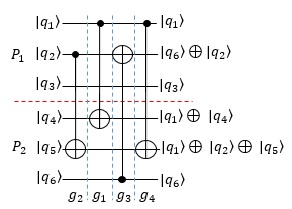
\includegraphics[width=50mm]{heuristic 1b}}
\subfigure {\label{b} 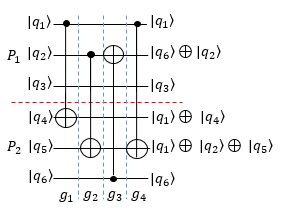
\includegraphics[width=50mm]{heuristic 1a}}
\subfigure {\label{c} 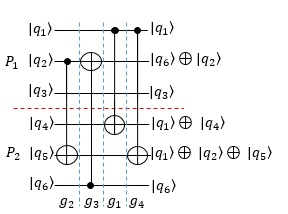
\includegraphics[width=50mm]{heuristic 1c}}
\caption{مثالی از روش ابتکاری $I$}
\label{heuristicIe}
\end{figure}
\item
روش ابتکاری دوم:
در روش دوم، ستون $i$ از ماتریس $C$ با ستون‌های مجاور خود $i+1 $ و $i+2 $ مقایسه می‌گردد. دو ستون کنار هم دارای یکی از سه حالت زیر هستند:
\begin{itemize}
\item
حالت ترکیب \LTRfootnote{\lr{Composition state}}: چنانچه در دوستون مجاور در سطر $i$ دو عنصر غیر صفر وجود داشته باشد، به اين معنا که این دو دروازه در کیوبیت شماره‌ی $q_i$ مشترک بوده و این دو ستون می‌توانند با یکدیگر ترکیب شوند. 
%\begin{equation}
%\text{if} \quad C[i][j]==C[i][j+1] \Rightarrow C[i][j]=max(C[i][j],C[i][j+1]) \& \quad \text{remove column j+1}
%\end{equation}
\item
حالت بلاک\LTRfootnote{\lr{Block state}}: چنانچه دو ستون پشت سرهم از ماتريس $C$ در سطر $i$ ام دارای دو عنصر غیر صفر با برچسب‌های متفاوت باشند، این دو ستون با یکدیگر ترکیب شده و مقدار برچسب ستون جدید به حالت $B$ تغییر مقدار می‌دهد. این وضعیت به آن معنی است که دو دروازه‌ی \lr{CNOT} پشت سرهم در یک کیوبیت مشترک بوده و برچسب آن‌ها متفاوت است. به‌عبارتی کیوبیت کنترلی یکی از دروازه‌ها کیوبیت هدف دیگری و یا بالعکس می‌باشد.
\item

حالت جابجاپذیر\LTRfootnote{\lr{Commutativity state}}: چنانچه دو ستون پشت سرهم در ماتریس در هیچ سطری دارای مقداری همزمان غیر صفر نباشند، این دو ستون می توانند با یکدیگر جابجا شوند. به عبارتی در هیج کیوبیت با یکدیگر اشتراک نداشته و از یکدیگر مستقل می‌باشند.
\end{itemize}
در شکل \ref{threestate} هر سه حالت ترکیب، بلاک و جابجا پذیر نشان داده شده است. الگوریتم 5 چگونگی اجرای روش ابتکاری $II$ را در جهت کاهش تعداد دورنوردی‌های کوانتومی نشان می‌دهد. این الگوریتم یکبار از سمت چپ ماتریس $C$ شروع به پردازش نموده و رو به جلو حرکت می‌کند. پس از آن، از انتهای ماتریس $C$ شروع نموده و در جهت رو به عقب حرکت نموده و عملیات بالا در جهت رو به عقب تکرار می‌شود. اين عمليات تا زماني ادامه مي‌يابد كه ابعاد ماتريس $C$ كاهش پيدا نیابد.

 \begin{figure}
\centering     
\subfigure[حالت ترکیب]{\label{state1}\includegraphics[width=30mm]{composition}}
\subfigure[حالت بلاک]{\label{state2}\includegraphics[width=30mm]{block}}
\subfigure[حالت جابجاپذیر]{\label{state3}\includegraphics[width=30mm]{commu}}
\caption{سه حالت بیان شده}
\label{threestate}
\end{figure}







\begin{algorithm}[t]
{
\fontsize{9}{1}
\caption{$\text{: الگوریتم  ابتکاری دوم}$}
\begin{algorithmic}[5]
\begin{latin}
\Function {Heuristic II} { Matrix C}
\State\textcolor[rgb]{0.00,0.50,1.00}{ $\triangleright$ Input: Matrix C}
\State\textcolor[rgb]{0.00,0.50,1.00}{ $\triangleright$ Output: Optimized Connectivity Matrix}
\State $Plength\leftarrow 1$;
\State $Tlength\leftarrow 0;$

\While {$C.length< PCM.length$ }
\State $PCM\leftarrow C;$
\For{ $i=0 : TCM.length()$}
 \If {$C_{i}$  and $C_{i+1}$  in Composition Status}
  \State{$C_{i}$=Composition($C_{i},C_{i+1};$)}
 \EndIf
  \If {$C_i$  and $C_{i+1}  in Block Status$}
  \State{$C_{i}$=Block($C_{i},C_{i+1};$)}
 \EndIf
 \If {$C[i]$  and $C[i+1]$  in commute Status}
  \State{$TCM\leftarrow C;$}
  \State {$swap(C_i,C_{i+1});$}
  \If{$C_i$ and $C_{i+1}$ Not in composition or Block state}
      \State{$C\leftarrow TCM;$}
  \EndIf
 \EndIf
\EndFor
\For{i=C.length()-1: 1}
 \If {$C_{i}$  and $C_{i-1}$  in Composition Status}
  \State{$C_{i-1}$=Composition($C_{i},C_{i-1}$);}
 \EndIf
  \If {$C_i$  and $C_{i-1}$  in Block Status}
  \State{$C_{i-1}$=Block($C_{i},C_{i-1});$}
 \EndIf
 \If {$C_i$  and $C_{i-1}$  in commute Status}
  \State{$TCM\leftarrow C;$}
  \State {$swap(C_i,C_{i-1});$}
  \If{$C_i$ and $C_{i-1}$ Not in composition or Block state}
      \State{$C\leftarrow TCM;$}
  \EndIf
 \EndIf
\EndFor
\EndWhile
\State{$N_t\leftarrow teleportationnum(C)$}
\State {Return $N_t$;}
\EndFunction
\end{latin}
\end{algorithmic}
}
\end{algorithm}

\end{itemize}
\subsection{ بهینه‌سازی سطح دوم جهت كاهش دورنوردي‌ها در چند زیر سیستم}


\begin{algorithm}
{
\caption{$\text{:الگوریتم اصلی جهت بهینه‌سازی تعداد دوربری‌های کوانتومی در سطح دوم برای چند سیستم }$}
\fontsize{9}{1}
\begin{algorithmic}[1]
\begin{latin}
\Function{Main algorithm} {Matrix C, Array P}
\State\textcolor[rgb]{0.00,0.50,1.00}{ $\triangleright$ Input: Matrix C, Array P}
\State\textcolor[rgb]{0.00,0.50,1.00}{ $\triangleright$ Output:Number of teleportations}
\State {$run$=\{0\};}
\State $N_t\leftarrow 0;$
\For {$s=1:s\leq N_{g} $ }
\If {$g_{s}$ \textrm{is a single qubit or local two-qubit gate}}
\State {$run[s]=1;$}
\Else
\If {$run[s]== 0$} \State\textcolor[rgb]{0.00,0.50,1.00}{ $\triangleright$ $g_{s}$ is a non-local gate}
\State {$run[s]==1;$}
\State $N_t\leftarrow N_t+1;$
\State{[$index_{1,s},index_{2,s}]=Find\_qubits(g_s);$}
\State{$q\_teleport \leftarrow index_{1,s};$}
\State{$P_{q\_teleport}\leftarrow P_{index_{2,s}};$}
\State{ $g_{d} \leftarrow$ \textrm{Find the first gate applied on q\_teleport and another qubit be located in} $P_{q\_teleport };$}
\State {$run[d]=Eexecute(g\_s,g\_d,q\_teleport);$}
\EndIf
\EndIf
\EndFor
\EndFunction
\end{latin}
\end{algorithmic}
}
\end{algorithm}


در این الگوریتم آرایه‌ای به نام $run$ ّبه اندازه‌ی تعداد دروازه‌های مدار در نظر گرفته می‌شود که مقدار $run[i]$ بیانگر حالت اجرای دروازه‌ی $i$ می‌باشد که دارای مقدار 0 (در صورت عدم اجرای دروازه‌ی $i$ام) و مقدار 1 (در صورت اجرای دروازه‌ی $i$ام) می‌باشد. دروازه‌ها یا همان ستون‌های ماتریس  $C$ از سمت چپ به راست با اندیس $s$ مورد بررسی قرار می‌گیرند. این دروازه‌ها در یکی از حالات زیر قرار دارند:
\begin{itemize}
\item
ستون $s$ از ماتریس $C$ بیانگر یک دروازه‌ی تک کیوبیتی است، در این صورت این دروازه اجرا شده و $run[s]=1 $ مقداردهی می‌گردد.
\item
ستون $s$ از ماتریس $C$ بیانگر یک دروازه‌ی محلی است، در این صورت این دروازه اجرا شده و $run[s]=1 $ مقداردهی می‌گردد.
\item
ستون $s$ بیانگر دروازه‌ی سراسری است و برای اجرا نیاز به دو دورنوردی کوانتومی دارد.
\end{itemize}
 در دو مورد اول دروازه $s$ بدون بررسی اجرا می‌گردد. اما در مورد سوم دروازه‌ی $s$ جهت اجرا نیاز به دو دورنوردی کوانتومی دارد (یکی برای رفتن کیوبیت از مبدا به مقصد و دیگری جهت بازگشت آن). فرض شود دروازه‌ی $g_s=(index_{1,s},index_{2,s})$ دارای دو کیوبیت $index_{2,s}$ و $index_{1,s}$ بوده و یکی از کیوبیت‌هایش که آن‌را $q\_teleport$ می‌نامیم، جهت اجرا به افراز مقصد دورنورد شود. در نتیجه $P_{q\_teleport}$ به شماره افرازی که $q\_teleport$ دورنوردی می‌شود، تغییر می‌یابد. سپس الگوریتم کل مدار را جستجو نموده تا دروازه‌ی اجرا نشده‌ای مانند $d$ بیابد که برای اجرا شدن نیاز به $q\_teleport$ داشته باشد. فرض شود دروازه‌ی $g_{d} (index_{1,d},index_{2,d})$ اولین دروازه‌ی سراسری باشد که دارای یکی از شرایط زیر است:

\begin{itemize}
\item
یکی از کیوبیت‌های  $index_{1,d}$ یا  $index_{2,d}$ برابر با $q\_teleport$ باشد.
\item 
کیوبیت دیگر آن در $P_{q\_teleport}$ قرار گرفته باشد.
\end{itemize}

\begin {figure*}[h]
\begin{center}
\begin{tikzpicture}
\node at (0,0) (q1) {\ket{q_{1}}};
\node at (0,-1) (q2) {\ket{q_{2}}};
\node at (0,-2) (q3) {\ket{q_{3}}};
\node at (0,-3) (q4) {\ket{q_{4}}};
\node at (0,-4) (q5) {\ket{q_{5}}};
\node at (0,-5) (q6) {\ket{q_{6}}};

% Column 2
\node[control] (c20) at (2,0) {} ;edge [-] (q1);
\node[operator] (r25) at (2,-5) {} ;edge [-] (q6);
\draw[-] (c20) -- (2,-5.3);

\node[operator] (c50) at (5,0) {} ;edge [-] (q1);
\node[control] (r53) at (5,-3) {} ;edge [-] (q4);
\draw[-] (r53) -- (5,0.3);

\node[operator] (r80) at (8,0) {} ;edge [-] (q1);
\node[control] (c84) at (8,-4) {} ;edge [-] (q6);
\draw[-] (8,0.3) -- (c84);

%gate
\node (end1) at (9,0) {} edge [-] (q1);\node (end2) at (9,-1) {} edge [-] (q2); \node (end3) at (9,-2) {} edge [-] (q3); \node (end4) at (9,-3) {} edge [-] (q4); \node (end4) at (9,-4) {} edge [-] (q5); \node (end4) at (9,-5) {} edge [-] (q6);
\node at (2,-6) {$g_{s}$}; \node at (5,-6) {$g_{k}$}; \node at (8,-6) {$g_{d}$};
%part
\draw [line1,dashed](-1,-3.5)-- (9.5,-3.5);\draw [line1,dashed](-1,-1.5)-- (9.5,-1.5);\draw [->] (c20) to [out=200, in=150,color=rgb] (r25); \node at (10,0) {$P_{1}$}; \node at (10,-2) {$P_{2}$}; \node at (10,-4) {$P_{3}$};\node at(2,0.5) {\small{\rl{ دورنورد شدن کیوبیت \ket{q_1} به افراز $P_3$}}};
\end{tikzpicture}
\end{center}
\caption{دورنورد شدن $q_{1}$ به افراز $P_{3}$ و بررسی دروازه‌ی                                                                                                                                                                                                                                                                                                                                                                                                                                                                                                                                                                                                                                                                                                                                                $g_{d}$ }
\label{figure4}
\end{figure*}
برای نمونه در مدار شکل \ref{figure4}، با دورنوردي شدن کیوبیت $q_1 $ از افراز $P_1 $ به افراز $P_3 $ اولین دروازه‌ی سراسری که در این کیوبیت با دروازه‌ی $g_s$ اشتراک دارد، دروازه‌ی $g_d$ می‌باشد. جهت بررسی اجرای این دروازه، تابعی بازگشتی به نام $Execute(g_{s},g_{d},q\_teleport)$ معرفی شده که اجرای دروازه‌ی $g_d$ را با دورنورد شدن $q\_teleport$ بررسی می‌کند. برای این تابع یکی از سه حالت زیر می‌تواند اتفاق بیفتد:
\begin{itemize}
\item
تعدادی دروازه‌ی اجرا نشده بین دروازه‌های $g_{s}$ و $g_{d}$ وجود داشته به‌طوری‌که این دروازه‌ها نتوانند قبل از اجرای $g_{d}$ اجرا شوند و اجرای دروازه‌ی $g_{d}$ به آن‌ها وابسته باشد. در این صورت این تابع مقداری  \lr{False} بر می‌گرداند. فرض شود که در ماتریس $C$ ستون $k (s < k <d)$ بیانگر $g_{k} (index_{1,k},index_{2,k})$ اولین دروازه‌ی اجرا نشده و سراسری قبل از ستون $d$ باشد. بنابراین در ستون $k$ام از ماتریس دو سطر غیرصفر $index_{1,k}$ و  $index_{2,k}$ وجود دارد. این شرایط در معادله‌ی \ref{eq11} نشان داده شده است.

\begin{figure}[htbp]
\centering
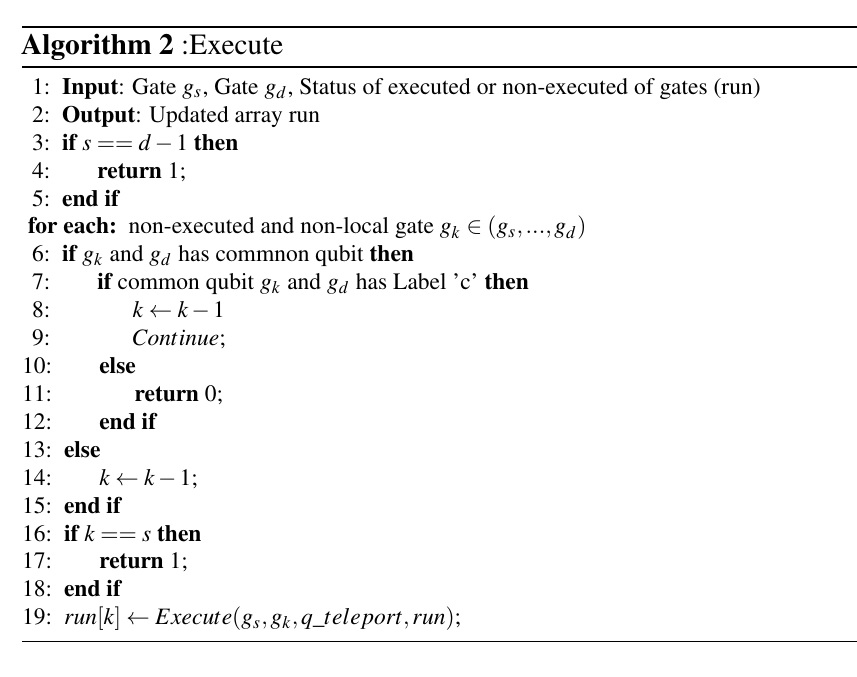
\includegraphics[scale=0.7]{execute.jpg}
\end{figure}



\begin{figure}[htbp]
\centering     
\subfigure[]{\label{a}\begin{tikzpicture}
\node at (0,0) (q1) {\ket{q_{1}}};
\node at (0,-1) (q2) {\ket{q_{2}}};
\node at (0,-2) (q3) {\ket{q_{3}}};
\node at (0,-3) (q4) {\ket{q_{4}}};
\node at (0,-4) (q5) {\ket{q_{5}}};
\node at (0,-5) (q6) {\ket{q_{6}}};

% Column 2
\node[control] (c20) at (2,0) {} ;edge [-] (q1);
\node[operator] (r25) at (2,-5) {} ;edge [-] (q6);
\draw[-] (c20) -- (2,-5.3);

\node[control] (c50) at (5,0) {} ;edge [-] (q1);
\node[operator] (r53) at (5,-3) {} ;edge [-] (q4);
\draw[-] (5,-3.3) -- (c50);

\node[operator] (r80) at (8,0) {} ;edge [-] (q1);
\node[control] (c84) at (8,-4) {} ;edge [-] (q6);
\draw[-] (8,0.3) -- (c84);

%gate
\node (end1) at (9,0) {} edge [-] (q1);\node (end2) at (9,-1) {} edge [-] (q2); \node (end3) at (9,-2) {} edge [-] (q3); \node (end4) at (9,-3) {} edge [-] (q4); \node (end4) at (9,-4) {} edge [-] (q5); \node (end4) at (9,-5) {} edge [-] (q6);
\node at (2,-6) {$g_{s}$}; \node at (5,-6) {$g_{k}$}; \node at (8,-6) {$g_{d}$};
%part
\draw [line1,dashed](-1,-3.5)-- (9.5,-3.5);\draw [line1,dashed](-1,-1.5)-- (9.5,-1.5);\draw [->] (c20) to [out=200, in=150,color=rgb] (r25); \node at (10,0) {$P_{1}$}; \node at (10,-2) {$P_{2}$}; \node at (10,-4) {$P_{3}$};\node at(2,0.5) {\small{\rl{ دورنورد شدن کیوبیت \ket{q_1} به افراز $P_3$}}};
\end{tikzpicture}
}
%\medskip

\subfigure[]{\label{b}\begin{tikzpicture}
\node at (0,0) (q1) {\ket{q_{1}}};
\node at (0,-1) (q2) {\ket{q_{2}}};
\node at (0,-2) (q3) {\ket{q_{3}}};
\node at (0,-3) (q4) {\ket{q_{4}}};
\node at (0,-4) (q5) {\ket{q_{5}}};
\node at (0,-5) (q6) {\ket{q_{6}}};

% Column 2
\node[control] (c20) at (2,0) {} ;edge [-] (q1);\node[operator] (r25) at (2,-5) {} ;edge [-] (q6);\draw[-] (c20) -- (2,-5.3);
\node[operator] (c50) at (5,0) {} ;edge [-] (q1);\node[control] (r53) at (5,-3) {} ;edge [-] (q4);\draw[-] (r53) -- (5,0.3);
\node[control] (c80) at (8,0) {} ;edge [-] (q1);\node[operator] (r84) at (8,-4) {} ;edge [-] (q6);\draw[-] (8,-4.3) -- (c80);

%gate
\node (end1) at (9,0) {} edge [-] (q1);\node (end2) at (9,-1) {} edge [-] (q2); \node (end3) at (9,-2) {} edge [-] (q3); \node (end4) at (9,-3) {} edge [-] (q4); \node (end4) at (9,-4) {} edge [-] (q5); \node (end4) at (9,-5) {} edge [-] (q6);
\node at (2,-6) {$g_{s}$}; \node at (5,-6) {$g_{k}$}; \node at (8,-6) {$g_{d}$};
%part
\draw [line1,dashed](-1,-3.5)-- (9.5,-3.5);\draw [line1,dashed](-1,-1.5)-- (9.5,-1.5);\draw [->] (c20) to [out=200, in=150,color=rgb] (r25); \node at (10,0) {$P_{1}$}; \node at (10,-2) {$P_{2}$}; \node at (10,-4) {$P_{3}$};\node at(2,0.5) {\small{\rl{ دورنورد شدن کیوبیت \ket{q_1} به افراز $P_3$}}};
\end{tikzpicture}}
\end{figure}
\begin{figure}
\centering
\subfigure[]{\label{c}\begin{tikzpicture}
\node at (0,0) (q1) {\ket{q_{1}}};
\node at (0,-1) (q2) {\ket{q_{2}}};
\node at (0,-2) (q3) {\ket{q_{3}}};
\node at (0,-3) (q4) {\ket{q_{4}}};
\node at (0,-4) (q5) {\ket{q_{5}}};
\node at (0,-5) (q6) {\ket{q_{6}}};

% Column 2
\node[control] (c20) at (2,0) {} ;edge [-] (q1);\node[operator] (r25) at (2,-5) {} ;edge [-] (q6);\draw[-] (c20) -- (2,-5.3);
\node[control] (c52) at (5,-2) {} ;edge [-] (q1);\node[operator] (r54) at (5,-4) {} ;edge [-] (q4);\draw[-] (5,-4.3) -- (c52);
\node[control] (c80) at (8,0) {} ;edge [-] (q1);\node[operator] (r84) at (8,-4) {} ;edge [-] (q6);\draw[-] (8,-4.3) -- (c80);

%gate
\node (end1) at (9,0) {} edge [-] (q1);\node (end2) at (9,-1) {} edge [-] (q2); \node (end3) at (9,-2) {} edge [-] (q3); \node (end4) at (9,-3) {} edge [-] (q4); \node (end4) at (9,-4) {} edge [-] (q5); \node (end4) at (9,-5) {} edge [-] (q6);
\node at (2,-6) {$g_{s}$}; \node at (5,-6) {$g_{k}$}; \node at (8,-6) {$g_{d}$};
%part
\draw [line1,dashed](-1,-3.5)-- (9.5,-3.5);\draw [line1,dashed](-1,-1.5)-- (9.5,-1.5);\draw [->] (c20) to [out=200, in=150,color=rgb] (r25); \node at (10,0) {$P_{1}$}; \node at (10,-2) {$P_{2}$}; \node at (10,-4) {$P_{3}$};\node at(2,0.5) {\small{\rl{ دورنورد شدن کیوبیت \ket{q_1} به افراز $P_3$}}};
\end{tikzpicture}
}
\subfigure[]{\label{d}\begin{tikzpicture}
\node at (0,0) (q1) {\ket{q_{1}}};
\node at (0,-1) (q2) {\ket{q_{2}}};
\node at (0,-2) (q3) {\ket{q_{3}}};
\node at (0,-3) (q4) {\ket{q_{4}}};
\node at (0,-4) (q5) {\ket{q_{5}}};
\node at (0,-5) (q6) {\ket{q_{6}}};

% Column 2
\node[control] (c20) at (2,0) {} ;edge [-] (q1);\node[operator] (r25) at (2,-5) {} ;edge [-] (q6);\draw[-] (c20) -- (2,-5.3);
\node[operator] (c52) at (5,-2) {} ;edge [-] (q1);\node[control] (r54) at (5,-4) {} ;edge [-] (q4);\draw[-] (5,-1.7) -- (r54);
\node[control] (c80) at (8,0) {} ;edge [-] (q1);\node[operator] (r84) at (8,-4) {} ;edge [-] (q6);\draw[-] (8,-4.3) -- (c80);

%gate
\node (end1) at (9,0) {} edge [-] (q1);\node (end2) at (9,-1) {} edge [-] (q2); \node (end3) at (9,-2) {} edge [-] (q3); \node (end4) at (9,-3) {} edge [-] (q4); \node (end4) at (9,-4) {} edge [-] (q5); \node (end4) at (9,-5) {} edge [-] (q6);
\node at (2,-6) {$g_{s}$}; \node at (5,-6) {$g_{k}$}; \node at (8,-6) {$g_{d}$};
%part
\draw [line1,dashed](-1,-3.5)-- (9.5,-3.5);\draw [line1,dashed](-1,-1.5)-- (9.5,-1.5);\draw [->] (c20) to [out=200, in=150,color=rgb] (r25); \node at (10,0) {$P_{1}$}; \node at (10,-2) {$P_{2}$}; \node at (10,-4) {$P_{3}$};\node at(2,0.5) {\small{\rl{ دورنورد شدن کیوبیت \ket{q_1} به افراز $P_3$}}};
\end{tikzpicture}
}
\caption{مدار کوانتومی ارائه شده با پنج دروازه و چهار کیوبیت. چهار حالتی که منجر به بازگرداندن \lr{False} در تابع می‌شود.}
\end{figure} 

این معادله بیان می‌کند دروازه‌های $g_{k}$ و $g_{d}$ در یک کیوبیت با برچسب‌های متفاوت مشترک بوده و یا اینکه در کیوبیت مشترک دارای برچسب \lr{`$t$'} مي‌باشند. همچنین کیوبیت دیگر آن‌ها در دو افراز متفاوت قرار داشته باشد. در این صورت دروازه‌ی $g_{d}$ از لحاظ اجرایی وابسته به اجرای دروازه‌ی $g_{k}$ است. و از آنجایی که دروازه‌ی $g_{k}$ جهت اجرا نیاز به یک دورنوردی دارد، در نتیجه دروازه‌‌ی $g_{d}$ نمی‌تواند اجرا شود و این تابع مقداری \lr{False} برمی‌گرداند. مدارات \ref{a} تا \ref{d} دارای این شرایط می‌باشند. در این مدارات، کیوبیت $q_{1}$ از افراز $P_{1}$ به افراز $P_{3}$ دورنورد می‌گردد. در نتیجه اولین دروازه‌ی سراسری اجرا نشده که نیاز به این کیوبیت دارد، دروازه‌ی $g_{d}$ می‌باشد. این دروازه جهت اجرا نیاز داشته که بین دروازه‌های $g_{d}$ و $g_{s}$ محدودیت‌های پیش نیازی رعایت شده باشد. پس از بازگشت به عقب اولین دروازه‌ی اجرا نشده‌ی سراسری مانند $g_{k}$ وجود دارد که اجرای $g_{d}$ به اجرای آن وابسته است. در نتیجه دروازه‌ی $g_{d}$ نمی‌تواند اجرا گردد و این تابع مقداری \lr{False} بر می‌گرداند.

چنان‌چه دروازه‌‌ی $g_{k}$ دروازه‌‌ای سراسری بوده که با دروازه‌ی $g_{d}$ دارای کیوبیت مشترک با برچسب \lr{`$c$'} باشد، آنگاه دروازه‌ی $g_d$ و $g_k$ از لحاظ اجرایی به یکدیگر وابستگی نداشته و بنابراین می‌توان از روی دروازه‌ی $g_k$ عبور نموده و اجرای آن را بررسی نکرد. این مفهوم در مدارات \ref{e} و \ref{ee} نشان داده شده است. در این حالت دروازه‌های $g_d$ و $g_k$ در کیوبیت $q_5 $ با برچسب \lr{`$c$'} مشترک بوده است. در این حالت می‌توان عدم اجرای دروازه‌ی $g_k$ را در نظر نگرفته و سایر دروازه‌های ماقبل از آن را بررسی نمود. به عبارتی وجود دروازه‌ی اجرا نشده‌ی $g_k$ تاثیری روی اجرا نشدن دروازه‌ی $g_d$ نداشته و باعث توقف تابع  \lr{Execute} نمی‌گردد. در نتیجه سایر دروازه‌های ما قبل از این دروازه تا رسیدن به دروازه‌ی $g_s$ بررسی می‌گردد. این شرایط در معادله‌ی \ref{eq12} بیان شده است.
\begin{equation}
\begin{split}
&index_{i,k}= index_{j,d}\quad \&\& \\ 
&({C[ {k,inpu{t_{i,k}}} ].label =C[{d,inpu{t_{j,d}}} ].label = `c`} ) \\
&\exists i,j \in\{1,2\}\\
\label{eq12}
\end{split}
\end{equation}

\begin{figure}[htbp]
\centering
\subfigure[]{\label{e}
\begin{tikzpicture}
\node at (0,0) (q1) {\ket{q_{1}}};
\node at (0,-1) (q2) {\ket{q_{2}}};
\node at (0,-2) (q3) {\ket{q_{3}}};
\node at (0,-3) (q4) {\ket{q_{4}}};
\node at (0,-4) (q5) {\ket{q_{5}}};
\node at (0,-5) (q6) {\ket{q_{6}}};

% Column 2
\node[control] (c20) at (2,0) {} ;edge [-] (q1);\node[operator] (r25) at (2,-5) {} ;edge [-] (q6);\draw[-] (c20) -- (2,-5.3);
\node[operator] (c52) at (5,-2) {} ;edge [-] (q1);\node[control] (r54) at (5,-4) {} ;edge [-] (q4);\draw[-] (5,-1.7) -- (r54);
\node[operator] (r80) at (8,0) {} ;edge [-] (q1);\node[control] (c84) at (8,-4) {} ;edge [-] (q6);\draw[-] (8,0.3) -- (c84);

%gate
\node (end1) at (9,0) {} edge [-] (q1);\node (end2) at (9,-1) {} edge [-] (q2); \node (end3) at (9,-2) {} edge [-] (q3); \node (end4) at (9,-3) {} edge [-] (q4); \node (end4) at (9,-4) {} edge [-] (q5); \node (end4) at (9,-5) {} edge [-] (q6);
\node at (2,-6) {$g_{s}$}; \node at (5,-6) {$g_{k}$}; \node at (8,-6) {$g_{d}$};
%part
\draw [line1,dashed](-1,-3.5)-- (9.5,-3.5);\draw [line1,dashed](-1,-1.5)-- (9.5,-1.5);\draw [->] (c20) to [out=200, in=150,color=rgb] (r25); \node at (10,0) {$P_{1}$}; \node at (10,-2) {$P_{2}$}; \node at (10,-4) {$P_{3}$};\node at(2,0.5) {\small{\rl{ دورنورد شدن کیوبیت \ket{q_1} به افراز $P_3$}}};
\end{tikzpicture}
}
\subfigure[]{\label{ee}\begin{tikzpicture}
\node at (0,0) (q1) {\ket{q_{1}}};
\node at (0,-1) (q2) {\ket{q_{2}}};
\node at (0,-2) (q3) {\ket{q_{3}}};
\node at (0,-3) (q4) {\ket{q_{4}}};
\node at (0,-4) (q5) {\ket{q_{5}}};
\node at (0,-5) (q6) {\ket{q_{6}}};

% Column 2
\node[control] (c20) at (2,0) {} ;edge [-] (q1);
\node[operator] (r25) at (2,-5) {} ;edge [-] (q6);
\draw[-] (c20) -- (2,-5.3);

\node[control] (c50) at (5,0) {} ;edge [-] (q1);
\node[operator] (r53) at (5,-3) {} ;edge [-] (q4);
\draw[-] (5,-3.3) -- (c50);

\node[control] (c80) at (8,0) {} ;edge [-] (q1);
\node[operator] (r84) at (8,-4) {} ;edge [-] (q6);
\draw[-] (8,-4.3) -- (c80);

%gate
\node (end1) at (9,0) {} edge [-] (q1);\node (end2) at (9,-1) {} edge [-] (q2); \node (end3) at (9,-2) {} edge [-] (q3); \node (end4) at (9,-3) {} edge [-] (q4); \node (end4) at (9,-4) {} edge [-] (q5); \node (end4) at (9,-5) {} edge [-] (q6);
\node at (2,-6) {$g_{s}$}; \node at (5,-6) {$g_{k}$}; \node at (8,-6) {$g_{d}$};
%part
\draw [line1,dashed](-1,-3.5)-- (9.5,-3.5);\draw [line1,dashed](-1,-1.5)-- (9.5,-1.5);\draw [->] (c20) to [out=200, in=150,color=rgb] (r25); \node at (10,0) {$P_{1}$}; \node at (10,-2) {$P_{2}$}; \node at (10,-4) {$P_{3}$};\node at(2,0.5) {\small{\rl{ دورنورد شدن کیوبیت \ket{q_1} به افراز $P_3$}}};
\end{tikzpicture}
}
\caption{دو حالتی که می‌توان اجرای دروازه‌ی $g_k$ را در نظر نگرفت.}
\end{figure}


%%%%%%%%%%%%%%%%%%%%5circuit
\item
چنانچه دروازه‌ی $g_k$ یک دروازه‌ی اجرا نشده‌ی تک کیوبیتی و یا دروازه‌ای محلی باشد که در یک کیوبیت با دروازه‌ی $g_d$ اشتراک داشته باشد، آنگاه این تابع به صورت بازگشتی اجرای دروازه‌ی $g_k$ را بررسی می‌نماید و به‌صورت $Execute(g_s,g_k, q_{teleport})$  فراخوانی می‌گردد.
\begin{figure}[htbp]
\centering
\subfigure[دروازه‌ی $g_k$ دروازه‌ای محلی و دو کیوبیتی بوده که اجرای دروازه‌ی $g_d$ به آن وابسته است]{\label{f}\begin{tikzpicture}
\node at (0,0) (q1) {\ket{q_{1}}};
\node at (0,-1) (q2) {\ket{q_{2}}};
\node at (0,-2) (q3) {\ket{q_{3}}};
\node at (0,-3) (q4) {\ket{q_{4}}};
\node at (0,-4) (q5) {\ket{q_{5}}};
\node at (0,-5) (q6) {\ket{q_{6}}};

% Column 2
\node[control] (c20) at (2,0) {} ;edge [-] (q1);\node[operator] (r25) at (2,-5) {} ;edge [-] (q6);\draw[-] (c20) -- (2,-5.3);
\node[control] (c55) at (5,-5) {} ;edge [-] (q1);\node[operator] (r54) at (5,-4) {} ;edge [-] (q4);\draw[-] (5,-3.7) -- (c55);
\node[operator] (r80) at (8,0) {} ;edge [-] (q1);\node[control] (c84) at (8,-4) {} ;edge [-] (q6);\draw[-] (8,0.3) -- (c84);

%gate
\node (end1) at (9,0) {} edge [-] (q1);\node (end2) at (9,-1) {} edge [-] (q2); \node (end3) at (9,-2) {} edge [-] (q3); \node (end4) at (9,-3) {} edge [-] (q4); \node (end4) at (9,-4) {} edge [-] (q5); \node (end4) at (9,-5) {} edge [-] (q6);
\node at (2,-6) {$g_{s}$}; \node at (5,-6) {$g_{k}$}; \node at (8,-6) {$g_{d}$};
%part
\draw [line1,dashed](-1,-3.5)-- (9.5,-3.5);\draw [line1,dashed](-1,-1.5)-- (9.5,-1.5);\draw [->] (c20) to [out=200, in=150,color=rgb] (r25); \node at (10,0) {$P_{1}$}; \node at (10,-2) {$P_{2}$}; \node at (10,-4) {$P_{3}$};\node at(2,0.5)  {\small{\rl{ دورنورد شدن کیوبیت \ket{q_1} به افراز $P_3$}}};
\end{tikzpicture}
}
\subfigure[دروازه‌ی $g_k$ دروازه‌ای تک کیوبیتی بوده که اجرای دروازه‌ی $g_d$ به آن وابسته است.]{\label{h}\begin{tikzpicture}
\node at (0,0) (q1) {\ket{q_{1}}};
\node at (0,-1) (q2) {\ket{q_{2}}};
\node at (0,-2) (q3) {\ket{q_{3}}};
\node at (0,-3) (q4) {\ket{q_{4}}};
\node at (0,-4) (q5) {\ket{q_{5}}};
\node at (0,-5) (q6) {\ket{q_{6}}};

% Column 2
\node[control] (c20) at (2,0) {} ;edge [-] (q1);\node[operator] (r25) at (2,-5) {} ;edge [-] (q6);\draw[-] (c20) -- (2,-5.3);
\node[hadamard] (h) at (5,-4) {H} ;
\node[operator] (r80) at (8,0) {} ;edge [-] (q1);\node[control] (c84) at (8,-4) {} ;edge [-] (q6);\draw[-] (8,0.3) -- (c84);

%gate
\node (end1) at (9,0) {} edge [-] (q1);\node (end2) at (9,-1) {} edge [-] (q2); \node (end3) at (9,-2) {} edge [-] (q3); \node (end4) at (9,-3) {} edge [-] (q4); \node (end4) at (9,-4) {} edge [-] (q5); \node (end4) at (9,-5) {} edge [-] (q6);
\node at (2,-6) {$g_{s}$}; \node at (5,-6) {$g_{k}$}; \node at (8,-6) {$g_{d}$};
%part
\draw [line1,dashed](-1,-3.5)-- (9.5,-3.5);\draw [line1,dashed](-1,-1.5)-- (9.5,-1.5);\draw [->] (c20) to [out=200, in=150,color=rgb] (r25); \node at (10,0) {$P_{1}$}; \node at (10,-2) {$P_{2}$}; \node at (10,-4) {$P_{3}$};\node at(2,0.5) {\small{\rl{ دورنورد شدن کیوبیت \ket{q_1} به افراز $P_3$}}};
\end{tikzpicture}
}

\end{figure}
\item

چنانچه هیچ درواز‌اه‌ای مانند $g_k$ با شرایط بیان شده در دو حالت قبل بین دروازه‌های $g_s$ و $g_d$ پیدا نگردید، می‌توان با دورنوردی نمودن کیوبیت $q\_{teleport}$ علاوه بر اجرای دروازه‌ی $g_s$ دروازه‌ی $g_d$ نیز اجرا گردد. در نتیجه $run[d]=1$ مقداردهي شده و تابع مقداری \lr{True} بر می‌گرداند.
\end{itemize}

\section{خلاصه}
در این فصل راه کار پیشنهادی برای توزیع مدار کوانتومی در چند زیر سیستم با رویکرد کاهش تعداد دورنوردی‌های کوانتومی و توزیع متوازن کیوبیت‌ها ارائه شد. به دلیل پیچیدگی بالای سیستم‌های کوانتومی، کاهش تعداد دورنوردی‌ها در یک سطح امری دشوار بود. جهت حل این مشکل، بهینه سازی دو سطحی در نظر گرفته شد. در سطح اول سعی گردید تا بتوان کیوبیت‌های مدار در تعدادی زیر سیستم به طور متوازن توزیع گردد به طوری که تعداد ارتباط‌ها لازم یا همان تعداد دروازه‌های سراسری بین زیر سیستم‌ها کاهش یابد. زمانی که یک کیوبیت از یک دروازه‌ی محلی از مبدا خود به مقصد مورد نظر دورنوردی می‌گردد، می‌تواند توسط سایر دروازه‌ها بدون برگشت آن به مقصد خود مورد استفاده قرار گیرد. این امر کاهش چشمگیری در  تعداد دورنوردی‌های مورد نیاز دارد. با در نظر گرفتن این ایده در سطح دوم، می‌توان تعداد دورنوردی‌ها را کاهش داد.

در این فصل، ابتدا یک مدل ریاضی با استفاده از برنامه ریزی خطی جهت افرازبندی مدار کوانتومی با هدف توزیع متوازن کیوبیت‌ها و تعداد دورنوردی‌های کوانتومی ارائه گردید. سپس الگوریتم‌های افرازبندی کیوبیت‌ها در دو زیر سیستم و چند زیر سیستم کوانتومی در سطح اول ارائه شد. سپس در سطح دوم تعدادی روش ابتکاری جهت کاهش تعداد دورنوردی‌های کوانتومی سطح دوم معرفی و اعمال گردید. 